\documentclass{report}
 
\usepackage[utf8]{inputenc} 
\usepackage[T1]{fontenc}      
\usepackage[top=3.5cm, bottom=3cm, left=4.0cm, right=4.0cm]{geometry}
\usepackage{graphicx}
\graphicspath{{figures/}{../figures}}

\begin{document}

\chapter{Fonctions de transfert, AO en régime linéaire - corrigé}

\newpage

\subsection*{Question de cours}

\subsubsection*{Formes canoniques}
Avec $x=\omega/\omega_0$ 
\begin{itemize}
	\item[•] Passe bas d'ordre 2 :
	\begin{equation}
		H(\omega)=\frac{H_0}{1+\frac{jx}{Q}-x^2}
	\end{equation}
	Résonance si $Q>1/\sqrt{2}$
	\item[•] Passe haut d'ordre 2 :
	\begin{equation}
		H(\omega)=\frac{-H_0x^2}{1+\frac{jx}{Q}-x^2}
	\end{equation}
	Résonance si $Q>1/\sqrt{2}$
	\item[•] Passe bande d'ordre 2 :
	\begin{equation}
		H(\omega)=\frac{H_0\frac{jx}{Q}}{1+\frac{jx}{Q}-x^2}
	\end{equation}
	Bande-passante : $\Delta\omega=\omega_0/Q$
\end{itemize}

\subsubsection*{Stabilité}
Un système est stable si la réponse à une entrée bornée est bornée. Autre critère : tous les coefficients de l'équation différentielle du régime libre sont de même signe, car le polynôme caractéristique a une racine de partie réelle positive et donc une solution est une exponentielle croissante.

\subsection*{AO idéal}

Un AO est idéal si : 
\begin{itemize}
	\item[-] Les courants d'entrées sont nuls ;
	\item[-] Différence de potentiel différentielle nulle en régime linéaire ;
	\item[-] Gain infini et retard nul (cf caractéristique idéale) en régime linéaire ;
	\item[-] Tension de sortie égale à $\pm V_{sat}$ en régime saturé.
	 
\end{itemize}


\section*{Correction Exercice 1}

\begin{itemize}
	\item[•] Amplificateur non-inverseur $u_s = \frac{R_1+R_2}{R_2}u_e$. Pour que $U_s = V_{nom}=2V_{max}$ il faut que le montage double la tension, cad $R_1=R_2$.
	\item[•]  Si $R_c=\infty$, alors le courant dans la charge $i_c$ est nul. Alors $P=u_si_s= \frac{R_1+R_2}{R_2^2}u_e^2$. L'AO consomme de l'énergie même s'il n'y a aucune puissance délivrée à la charge !
	\item[•] Soit $i_1$ le courant traversant $R_1$ et $R_2$. Alors la loi des nœuds donne : $i_s-i_1-ic=0$ (signe pris tq les puissances soient positives). On a alors :
	\begin{equation}
		P=u_si_s=\frac{R_1+R_2}{R_2^2}u_e^2+\frac{(R_1+R_2)^2}{R_2^2R_c}u_e^2
	\end{equation}
	\item[•] On prend $R_2\gg R_c$, le premier terme de dissipation de l'AO devient négligeable devant la puissance envoyée à la charge.
\end{itemize}

\section*{Correction exercice 2}
Fonction de transfert :
\begin{equation}
	H=\frac{u_s}{u_e}=\frac{R_1+R_2}{R}\frac{1+j\frac{R_1R_2}{R_1+R_2}(C_1+C_2)\omega}{(1+jR_1C_1\omega)(1+jR_2C_2\omega)}=H_0\frac{1+j\omega/\omega_0}{(1+j\omega/\omega_1)(1+j\omega/\omega_2)}
\end{equation}
donc $H_0=\frac{R_1+R_2}{R}$, $\omega_0=\frac{R_1+R_2}{R_1R_2(C_1+C_2)}$, $\omega_1=1/R_1C_1$ et $\omega_2=1/R_2C_2$

Diagramme de Bode : on décompose en somme des diagramme de Bode des différents produits.

\textbf{Cas $\omega_0<\omega_1<\omega_2$ :}
\begin{figure}[!h]
	\centering
	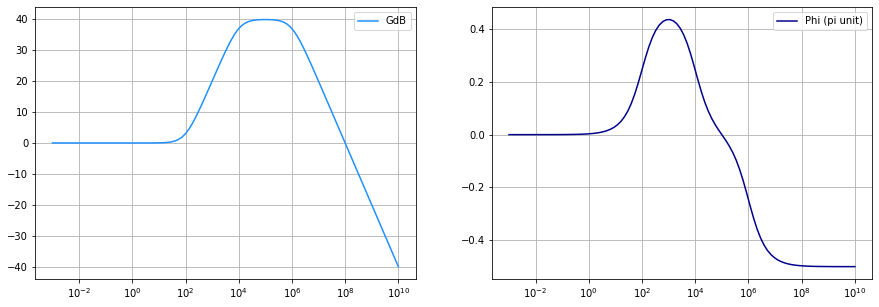
\includegraphics[width=0.8\linewidth]{exo2_0.png}
\end{figure}

\textbf{Cas $\omega_1<\omega_0<\omega_2$ :}
\begin{figure}[!h]
	\centering
	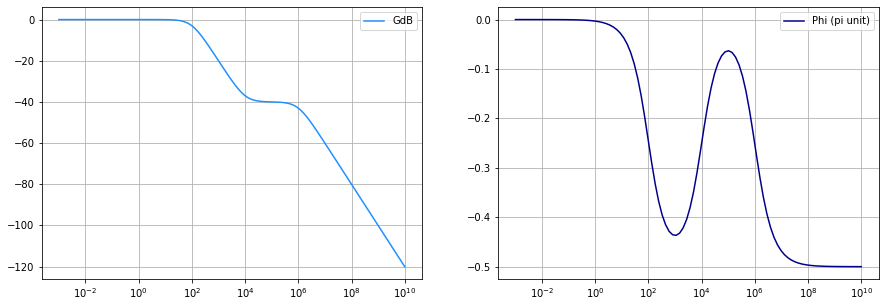
\includegraphics[width=0.8\linewidth]{exo2_1.png}
\end{figure}

\textbf{Cas $\omega_1<\omega_2<\omega_0$ :}
\begin{figure}[!h]
	\centering
	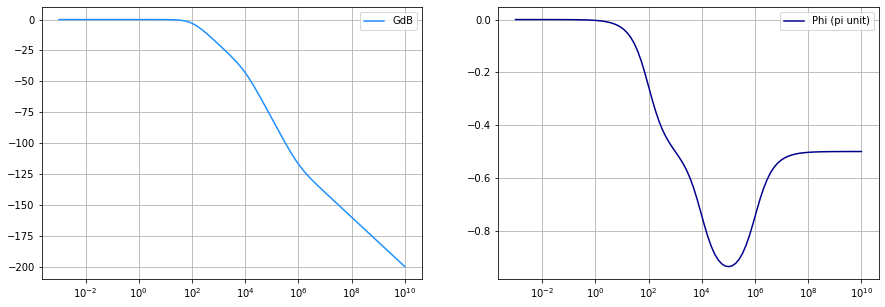
\includegraphics[width=0.8\linewidth]{exo2_2.png}
\end{figure}

\section*{Correction exercice 3}

Le courant de sortie est supposé nul.

\begin{itemize}
	\item[•] Comportement : BF, $u_e=u_s$ et HF, $u_e=u_s$, c'est un filtre passe bande
	
	\item[•]
		Pour la fonction de transfert, on fait une loi des nœuds en A (entre les 2 résistances du haut), en B (entre les 2 capa du milieu) et à la sortie :
	\begin{equation}
		(u_e-u_a)/R+(u_s-u_a)/R-j2C\omega u_a=0
	\end{equation}
	\begin{equation}
		(u_e-u_b)jC\omega+(u_s-u_b)jC\omega-u_b/R=0
	\end{equation}
	\begin{equation}
		(u_s-u_a)/R+-jC\omega(u_s-u_b)=0
	\end{equation}
	On trouve alors :
	\begin{equation}
		H =\frac{1+(jRC\omega)^2}{1+4jRC\omega + (jRC\omega)^2}
	\end{equation}
	
	\item[•]
	Diagramme de Bode :
Diagramme assymptotique :  $\forall \omega, H=0$ et pour $\omega=\omega_0=1/RC$, dirac à "l'envers" avec $H=-\infty$. C'est bien un coupe-bande.

	\item[•] Bande-passante :
	$G_{DB} = -20\log \sqrt{1+\left( \frac{4RC\omega}{1-R^2C^2\omega^2}\right) ^2}=-3$ 
	
	$\Rightarrow R^2C^2\omega^2 - 4RC\omega -1=0$
	alors : $\omega_{\pm}=\frac{\pm 2+\sqrt{5}}{RC}$
	
	AN : $\omega_- = 230$ Hz et $\omega_+ = 4230$ Hz
	
	\item[•] Question supplémentaire : 
	Le filtre supprime les harmonique 1 et 3. Le signal est un créneau, pour le tracer, on retire les 2 premières harmoniques d'un signal créneau.
\end{itemize}

\section*{Correction exercice 4}

\begin{itemize}
	\item[•]
	$H=\frac{1-jRC\omega}{1+jRC\omega}$. On remarque que $\mid H\mid=1$, mais que $\varphi=-2\arctan(RC\omega)$. On peut écrire alors $H$ sous la forme :
	\begin{equation}
		H=e^{-2j\arctan(RC\omega)}
	\end{equation}
C'est un filtre déphaseur.

	\item[•]
	Dans l'espace de fourier, pour un signal quelconque d'entrée $e(t)=\sum_k A_k e^{jk\omega_0 t}$, la sortie est :
	\begin{equation}
		s(t)=\sum_k A_k e^{jk\omega_0 t+j\varphi(k\omega_0)}
	\end{equation}
	Si $\omega\ll RC$, alors $\varphi(\omega)\longrightarrow-2RC\omega$ et que toutes les harmoniques valident cette condition (ex : signal triangulaire, avec une décroissance rapide de l'amplitude des harmoniques) :
	\begin{equation}
		s(t)=\sum_k A_k e^{jk\omega_0 (t-2RC)}=e(t-\tau)
	\end{equation}
	
	\item[•] $\cos^3(\omega t)=\frac{1}{4}(3\cos(\omega t) + \cos(3\omega t))$.
	Le signal de sortie sera donc : 
	\begin{equation}
	U_s(t) = \frac{1}{4}\left[ 3\cos(\omega t - 2\arctan(\omega/\omega_0)) + \cos(3\omega t - 2\arctan(3\omega/\omega_0))\right] 
	\end{equation}
	Pour $\omega = \frac{\omega_{0}}{3}$, on a une déformation du signal car la condition précédente sur le retard n'es tpas vérifiée. Pour $\omega=10^{-2}\omega_0$, le signal est retardé d'une durée $\tau=2/\omega_0=2RC$.
	
	\item[•] Pour $t<0$, le condensateur est déchargé donc $u_e(t)=u_s(t)=0$. Pour $t\geq0$, le condensateur se charge donc $u_-(t) = E(1-e^{-t/RC})$, et alors :
	\begin{equation}
		u_s(t)=2E(1-e^{-t/RC}) - E
	\end{equation}
	Le signal finit bien par "redevenir" celui d'entrée (car $H=1$) mais un retard. Attention, ici c'est une transformation de Fourier et non une série de Fourier qu'il faut opérer. 
	
\end{itemize}

\subsection*{Correction exercice 5}

\begin{itemize}
	\item[•] $H = -jRC\omega$ cad $u_s(t) = -RC\frac{du_e}{dt}$. C'est un dérivateur.
	\item[•] En TF : $u_s = \varepsilon\frac{\mu_0}{1+j\tau\omega}$. Puis loi des nœuds, avec $\varepsilon=u_-$ :
	\begin{equation}
		H(j\omega) = \frac{-\mu_0jRC\omega}{1+\mu_0 + j\omega(\tau+RC)-RC\tau\omega^2}
	\end{equation}
	L'équation différentielle associée à tous ses coefficients du même signe, les solutions sont sinusoïdales donc bornées. 
	\item[•] En inversant les pôles, $\varepsilon=+u_-$. Cela revient à remplacer $\mu_0\leftarrow-\mu_0$. Le terme de dérivée 0 devient alors $1-\mu_0$ et est négatif donc la solution contient une partie exponentielle et diverge jusqu'à saturation.
	\item[•] C'est un filtre passe bande d'ordre 2 de pulsation $\omega_0=\sqrt{\frac{1+\mu_0}{RC\tau}}$
	Sous forme canonique, on a :
		\begin{equation}
		H(j\omega) = \frac{H_0}{1+jQ(x-\frac{1}{x})}
	\end{equation}
	avec $H_0=\frac{\mu_0RC}{\tau+RC}=-5,9\cdot10^3$ et $Q = \frac{\sqrt{(1+\mu_0)RC\tau}}{\tau+RC}=74$
	Ce filtre est dérivateur pour $x$ petit, cad $H\approx \frac{j\omega}{Q\omega_0}$. Cette condition est vérifiée jusqu'à $x\approx0,9$ cad $f=2\pi\omega\approx11$kHz.
\end{itemize}


\end{document}
